\documentclass{article}
\usepackage[a4paper, tmargin=2cm,rmargin=1.5in,lmargin=1.5in,margin=0.85in,bmargin=2cm,footskip=.2in]{geometry}
\usepackage{bookmark}
\usepackage{listings}
\usepackage{amsmath,amsfonts,amsthm,amssymb,mathtools}
\usepackage[italian]{babel}
\usepackage{graphicx}
\graphicspath{{img/},{py and pdf/}}

\usepackage{multirow}
\usepackage{subfloat}
\usepackage{wrapfig}
\usepackage{float}
\usepackage{caption}
\usepackage{setspace}
\usepackage{ragged2e}
\usepackage{longtable}
\usepackage[T1]{fontenc}
\usepackage{hyperref}
\title{\Huge{Misure di densità}}
\author{\large{Giosué Aiello}}
\date{\today}
\usepackage{xcolor}
\usepackage{titling}
\renewcommand\maketitlehooka{\null\mbox{}\vfill}
\renewcommand\maketitlehookd{\vfill\null}
\definecolor{codegreen}{rgb}{0,0.6,0}
\definecolor{codegray}{rgb}{0.5,0.5,0.5}
\definecolor{codepurple}{rgb}{0.58,0,0.82}
\definecolor{backcolour}{rgb}{0.95,0.95,0.92}
\usepackage{subcaption}
% Label format
\DeclareCaptionLabelFormat{custom}
{%
      \textsc{#1 \textbf{(#2)}}
}
% Separator style
\DeclareCaptionLabelSeparator{custom}{--}
% Caption format    
\DeclareCaptionFormat{custom}
{%
    #1#2 \small #3
}
\captionsetup{
	format=custom,
	labelformat=custom,
	labelsep=custom
}
\lstdefinestyle{code}{
    backgroundcolor=\color{backcolour},   
    commentstyle=\color{codegreen},
    keywordstyle=\color{magenta},
    numberstyle=\tiny\color{codegray},
    stringstyle=\color{codepurple},
    basicstyle=\ttfamily\footnotesize,
    breakatwhitespace=false,         
    breaklines=true,                 
    captionpos=b,                    
    keepspaces=true,                 
    numbers=left,                    
    numbersep=5pt,                  
    showspaces=false,                
    showstringspaces=false,
    showtabs=false,                  
    tabsize=2
}
\usepackage{xcolor}
\usepackage{hyperref}

\usepackage{hyperref}
\hypersetup{
    colorlinks=true,
    linkcolor=black,
    pdfborder={0 0 0},
	urlcolor=black,
}

\setlength{\parindent}{0pt}

% Configurazione dello stile per il codice Python
\usepackage{listings}
\usepackage{xcolor}

% Definizione dei colori
\definecolor{codegreen}{rgb}{0,0.6,0}
\definecolor{codegray}{rgb}{0.5,0.5,0.5}
\definecolor{codepurple}{rgb}{0.58,0,0.82}
\definecolor{backcolour}{rgb}{0.95,0.95,0.92}
\lstdefinestyle{mystyle}{
    backgroundcolor=\color{backcolour},   
    commentstyle=\color{codegreen},
    keywordstyle=\color{magenta},
    numberstyle=\tiny\color{codegray},
    stringstyle=\color{codepurple},
    basicstyle=\ttfamily\footnotesize,
    breakatwhitespace=false,         
    breaklines=true,                 
    captionpos=b,                    
    keepspaces=true,                 
    numbers=left,                    
    numbersep=5pt,                  
    showspaces=false,                
    showstringspaces=false,
    showtabs=false,                  
    tabsize=2,
    language=Python
}

\lstset{style=mystyle}


\begin{document}
	\begin{titlingpage}
    \begin{center}
        \vspace*{60pt} % Spazio dall'inizio della pagina

        {\Huge \textbf{\textsc{Calcolo di G}}} % Titolo in maiuscoletto
        \vspace{30pt} % Spazio dopo il titolo

        {\huge{Giosuè Aiello}} % Autore in corsivo e un po' più piccolo
        \vspace{20pt} % Spazio dopo l'autore

        {\large \today} % Data
    \end{center}
    
    \vfill % Riempie lo spazio verticale rimanente
\end{titlingpage}

\pagebreak
    \section{Scopo dell'esperienza}
    Lo scopo dell'esperienza è di misurare il valore dell’accelerazione gravitazionale $g$ sulla superficie terrestre. 
     
    
 \section{Premesse teoriche}    
    Il valore medio tabulato di riferimento è $g = 9.8 \, m/s^2$. È possibile misurare il rapporto fra la costante elastica $k$ di una molla e $g$ conoscendo l’allungamento della stessa rispetto alla posizione di equilibrio dovuto ad una massa appesa alla sua estremità. Infatti, per la legge di Hooke:
    \[
    F = k \cdot \Delta l = m \cdot g
    \]
    da cui segue
    \[
    k = \frac{m \cdot g}{\Delta l}
    \]

    Dove:
    \begin{itemize}
        \item $m_p$ è la massa del piattello appeso alla molla,
        \item $m_i$ è la massa appoggiata sul piattello,
        \item $l_0$ è la lunghezza della molla a riposo,
        \item $l_i$ è la lunghezza della molla dilatata.
    \end{itemize}

    Una molla è un corpo in grado di allungarsi e accorciarsi se gli viene applicata una forza e in seguito di ritornare alla propria forma naturale. Tramite la legge di Hooke sappiamo che essa reagisce esercitando una forza che reagisce alle sollecitazione subita longitudinalmente, in trazione o in compressione, lungo un asse $\hat{x}$
    \begin{equation}
        \vec{F_e} = - k \Delta l \hat{x}
    \end{equation}
    quindi si osserva che essa è direttamente proporzionale all'allungamento o alla compressione $\Delta l$ (che dimensionalmente ha come unità di misura quella di una lunghezza $[L]$) della molla dovuto alla sollecitazione e la costante di questa proporzionalità $k$ si chiama \emph{costante elastica della molla} (che invece dimensionalmente ha l'unità di misura di una forza diviso una lunghezza, dunque $\frac{[L][T]^{-2}[M]}{[L]} = [M][T]^{-2}$). \\
    La forza di gravità esercitata dalla Terra su un corpo che si trova sulla sua superficie è pari a
    $\vec{F} = m\vec{g}$
    dove $\vec{g}$ è l'accelerazione di gravità sulla superficie terrestre. È possibile stimare il valore di $g=|\vec{g}|$ misurando l'allungamento della molla dovuto all'azione di una massa appesa ad una estremità della molla, pertanto:
    \begin{equation}
        m|\vec{g}| = k \Delta l \implies |\vec{g}| = \frac{k}{m} \Delta l
        \label{secondo_modello}
    \end{equation}
    Tramite una stima della lunghezze $\Delta l$, $k$ e conoscendo la massa $m$ appesa possiamo stimare g. Per fare ciò, ci avvarremo della formula del periodo $T$ delle oscillazioni compiute dalla molla con la massa appesa
    \begin{equation}
        T = 2 \pi \sqrt{\frac{m}{k}}
    \end{equation}
    Da cui risulta che 
    \begin{equation}
        T^2 = \frac{4\pi^2}{k} m
        \label{primo_modello}
    \end{equation}


%------------------------------------------------------------------------------------------
%--------------------------------------------------------------------------------------------
    \section{Descrizione delle misure}
    La prima parte dell’esperienza consisterà nel misurare le dilatazioni di lunghezza $l_i - l_0$ prodotte dalle masse $m_i$. Successivamente dal grafico $l$-$m$ (il cui fit è una retta di coefficiente angolare $k$) otterremo una stima di $k$.

    Per ricavare $k$ (e quindi $g$) sfruttiamo la legge che esprime la dipendenza del periodo $T$ dalla massa appesa alla molla secondo la quale:
    \[
    T = 2\pi \sqrt{\frac{m}{k}}
    \]
    da cui
    \[
    k = \frac{4\pi^2 m}{T^2}
    \]

    \section{Apparato Sperimentale}
    L’apparato sperimentale necessario per effettuare l’esperienza (Fig. 1) consiste in una molla ed un supporto cui appenderla, un piattello e delle masse. Gli strumenti utilizzati sono un metro a nastro, un cronometro e una bilancia.

    \begin{figure}[H]
        \centering
        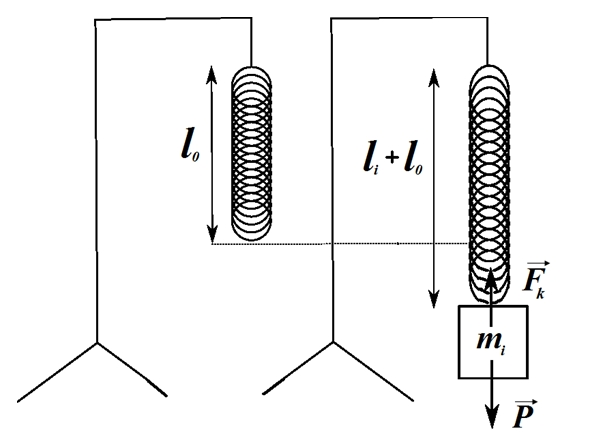
\includegraphics[width=0.5\textwidth]{fig1.jpg}
        \caption{Strumentazione utilizzata per l’esperimento}
        \label{fig:apparato}
    \end{figure}

    \section{Dati}
    Le misure di $l$ al variare della massa $m$ sono le seguenti:

    \begin{table}[H]
        \centering
        \begin{tabular}{|c|c|}
            \hline
            $m (kg)$ & $l (cm)$ \\
            \hline
            0.05 & 8.0 \\
            0.10 & 10.0 \\
            0.15 & 12.0 \\
            0.20 & 14.0 \\
            0.25 & 16.0 \\
            0.30 & 18.0 \\
            \hline
        \end{tabular}
        \caption{Misure di $l$ al variare di $m$}
        \label{tab:misure}
    \end{table}

    \section{Elaborazione dei Dati}
    Tramite i dati raccolti, si è potuto costruire il grafico della lunghezza $l$ al variare della massa $m$, come mostrato in Figura 2.

    \begin{figure}[H]
        \centering
        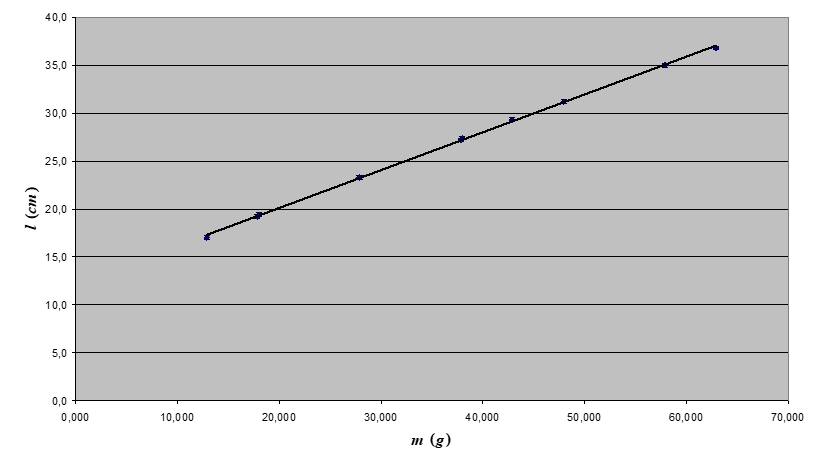
\includegraphics[width=0.5\textwidth]{fig2.jpg}
        \caption{Grafico della lunghezza $l$ al variare della massa $m$}
        \label{fig:grafico}
    \end{figure}

    Dal coefficiente angolare della retta che meglio interpola i dati sperimentali si è ottenuta una stima di $k = 0.40 \, N/m$.

    \section{Conclusioni}
    Con i dati sperimentali ottenuti e utilizzando le equazioni [3] e [5], abbiamo calcolato il valore di $g$ come $g = 9.81 \, m/s^2$, che risulta essere molto vicino al valore tabulato di riferimento $g = 9.8 \, m/s^2$.

    \begin{figure}[H]
        \centering
        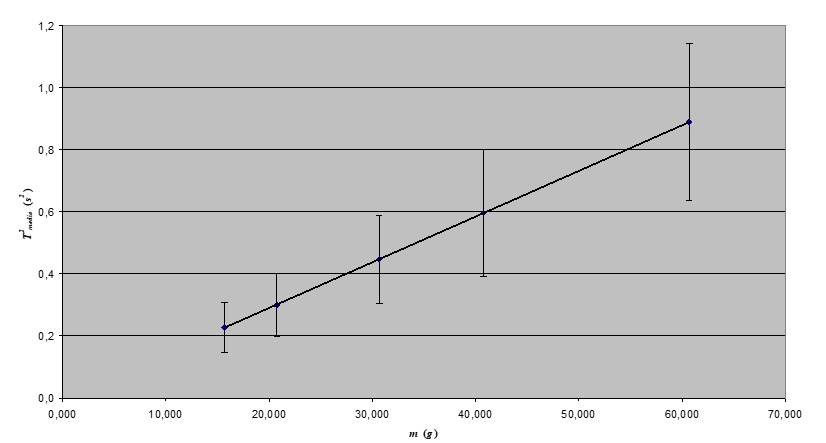
\includegraphics[width=0.5\textwidth]{fig3.jpg}
        \caption{Grafico dell'andamento del periodo $T$ al variare della massa $m$}
        \label{fig:periodo}
    \end{figure}

\end{document}

